% Data: completed presentation/ACTUAL_FOUR_LIVE_CONFIRMATION_CELLS.csv.
% Native TikZ only; no external plotting or experimental execution.
\begin{figure}[t]
\centering
\begingroup
\definecolor{resultblue}{HTML}{0072B2}
\definecolor{resultorange}{HTML}{D55E00}
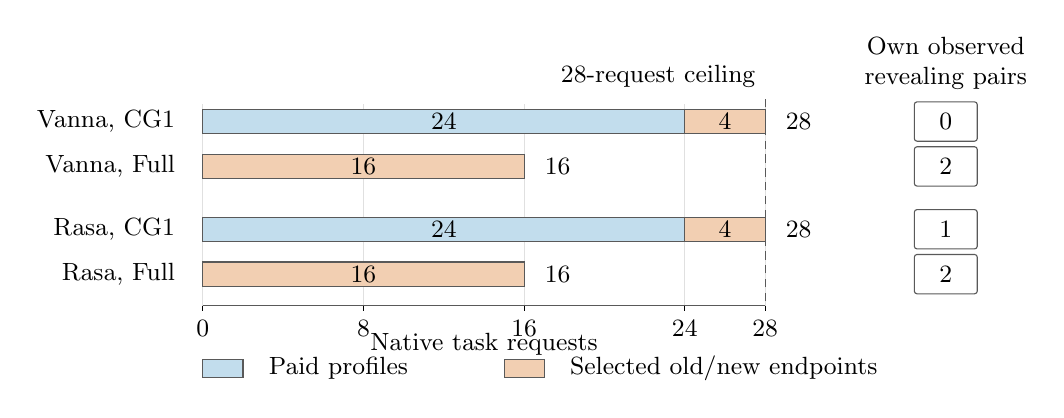
\begin{tikzpicture}[x=0.255cm,y=0.57cm,font=\small]
  \foreach \tick in {0,8,16,24,28} {
    \draw[black!12] (\tick,-0.1) -- (\tick,4.4);
    \draw (\tick,-0.1) -- (\tick,-0.22);
    \node[below] at (\tick,-0.22) {\tick};
  }
  \draw[black!65] (0,-0.1) -- (28,-0.1);
  \draw[black!65,densely dashed] (28,0) -- (28,4.5);
  \node[anchor=south east] at (28,4.55) {28-request ceiling};
  \node[align=center] at (37,5.3) {Own observed\\revealing pairs};
  % App/method, row, profiling, selected endpoints, own observed pair count.
  \foreach \method/\row/\profile/\selected/\pairs in {
    {Vanna, CG1}/4/24/4/0,
    {Vanna, Full}/3/0/16/2,
    {Rasa, CG1}/1.6/24/4/1,
    {Rasa, Full}/0.6/0/16/2} {
    \node[anchor=east] at (-0.9,\row) {\method};
    \pgfmathsetmacro{\total}{\profile+\selected}
    \ifnum\profile>0
      \filldraw[fill=resultblue!24,draw=black!65]
        (0,{\row-0.27}) rectangle (\profile,{\row+0.27});
      \node at ({\profile/2},\row) {\profile};
    \fi
    \filldraw[fill=resultorange!30,draw=black!65]
      (\profile,{\row-0.27}) rectangle (\total,{\row+0.27});
    \node at ({\profile+\selected/2},\row) {\selected};
    \node[anchor=west] at ({\total+0.55},\row)
      {\pgfmathprintnumber[precision=0]{\total}};
    \node[draw=black!65,rounded corners=1pt,minimum width=8mm,
      minimum height=5mm,fill=white] at (37,\row) {\pairs};
  }
  \node at (14,-0.96) {Native task requests};
  \filldraw[fill=resultblue!24,draw=black!65] (0,-1.7) rectangle (2,-1.3);
  \node[anchor=west] at (2.8,-1.5) {Paid profiles};
  \filldraw[fill=resultorange!30,draw=black!65] (15,-1.7) rectangle (17,-1.3);
  \node[anchor=west] at (17.8,-1.5) {Selected old/new endpoints};
\end{tikzpicture}
\endgroup
\caption{Fresh cold-start execution under the same 28-request ceiling.
Stacked bars separate paid profiles from selected old/new task invocations;
totals appear at the bar ends. Full paired retesting uses 16 requests, leaves
12 of its 28-request allowance unused, and observes
two revealing pairs per setting. CG1 uses 28 requests and observes zero in
Vanna and one in Rasa. Pair counts come from each method's own fresh executions;
they are not independent bugs or recall against another method's outcomes.
History is empty and judgments are exact. Rasa requests execute CPU application
paths rather than a generative provider.}
\Description{Four horizontal stacked bars compare native requests and each
method's own observed revealing pairs. Vanna CG1 uses 24 profile requests plus
4 selected endpoints, total 28, and observes 0 pairs. Rasa CG1 uses the same
24 plus 4 requests and observes 1 pair. Full retesting in each setting uses
0 profile requests plus 16 endpoints, total 16, and observes 2 pairs. All
methods have a 28-request ceiling.}
\label{fig:result-cold}
\end{figure}
